\documentclass[11pt]{article}
\usepackage[margin=1in]{geometry}
\usepackage[T1]{fontenc}
\usepackage[utf8]{inputenc}
\usepackage{lmodern}
\usepackage{microtype}
\usepackage{amsmath,amssymb,amsthm,mathtools,bm}
\usepackage{booktabs,multirow,array}
\usepackage{enumitem}
\usepackage{xcolor}
\usepackage{hyperref}
\usepackage{graphicx}
\usepackage{tikz}
\usepackage{pgfplots}
\usepackage{subcaption}
\usepackage{algorithm}
\usepackage{algpseudocode}
\usetikzlibrary{arrows.meta,positioning,calc,fit,backgrounds,shapes.geometric}
\pgfplotsset{compat=1.18}
\hypersetup{colorlinks=true,linkcolor=blue!60!black,citecolor=blue!60!black,urlcolor=blue!60!black}

\newcommand{\R}{\mathbb{R}}
\newcommand{\E}{\mathbb{E}}
\newcommand{\1}{\mathbf{1}}
\newcommand{\cvar}{\operatorname{CVaR}}
\newcommand{\diag}{\operatorname{diag}}
\newcommand{\softmax}{\operatorname{softmax}}
\newcommand{\proj}{\operatorname{Proj}}
\newcommand{\norm}[1]{\left\lVert #1 \right\rVert}
\newcommand{\abs}[1]{\left\lvert #1 \right\rvert}
\newcommand{\ip}[2]{\left\langle #1, #2 \right\rangle}
\newcommand{\ubar}{u_E}
\newcommand{\Aset}{\mathcal{A}_\rho}
\newcommand{\Qset}{\mathcal{Q}_\beta}
\newcommand{\Dset}{\Delta_K}
\newcommand{\Pperp}{P_\perp}
\newcommand{\bb}{\bar b}

\definecolor{accent}{RGB}{31,78,121}
\definecolor{accent2}{RGB}{0,128,128}
\definecolor{accent3}{RGB}{188,79,27}
\definecolor{softgray}{RGB}{245,247,250}

\theoremstyle{plain}
\newtheorem{theorem}{Theorem}[section]
\newtheorem{proposition}[theorem]{Proposition}
\newtheorem{corollary}[theorem]{Corollary}
\newtheorem{lemma}[theorem]{Lemma}
\theoremstyle{definition}
\newtheorem{definition}[theorem]{Definition}
\newtheorem{assumption}[theorem]{Assumption}
\theoremstyle{remark}
\newtheorem{remark}[theorem]{Remark}

\title{\vspace{-1.0em}\bfseries Global Canalized Souping:\\
A Principled Convex Theory of Post-hoc Domain Generalization from Source-Mixture Robustness}
\author{Anonymous Authors}
\date{}

\begin{document}
\maketitle

\begin{abstract}
Post-hoc domain generalization matters because it is one of the few robustness strategies that can be attached to a strong empirical-risk-minimization pipeline without retraining. A single training run, or a small set of completed runs, produces a bank of checkpoints, and one deployable model is chosen only after optimization has already finished. This regime is operationally attractive and empirically credible. Existing successful methods are commonly explained through flatness, locality, or diversity. We develop a local, assumption-explicit theory in which these phenomena appear from one common premise: a deployable post-hoc model should be robust to small signed tangent perturbations of source-mixture weights---and, in sufficiently local feasible regimes, to literal redistributions of source-support mass---while remaining safely mergeable inside a low-curvature region of weight space. The theorem-bearing object is a source-mixture robust risk over domain losses. The practical method is obtained by pushing that object through a second-order soup approximation on the full checkpoint bank, with no retained-family search, no grid search over supports, and no heuristic greedy subset construction. We prove an exact hidden-shift support-function identity, a target-risk upper bound that is explicitly conditional on a fixed target-side envelope assumption, a robust-envelope characterization of source CVaR, an observable-form convex upper bound for the deployed soup whose curvature constants come from local smoothness assumptions, interaction decompositions showing how diversity helps, and low-curvature corollaries showing how flat averaging enters the same local framework. The resulting method, Global Canalized Souping (GCS), solves one convex optimization over the entire checkpoint bank using source-domain held-out losses, observable checkpoint-domain loss profiles, and local checkpoint geometry. Accordingly, the theory should be read as a deterministic held-out-loss analysis, or as a population-risk analysis only after an additional generalization layer is supplied. The empirical panels included here are explicitly illustrative placeholders rather than measured results.\vspace{-0.25em}
\end{abstract}

\section{Introduction}
Domain generalization (DG) studies how to train a model on several source domains and deploy it on an unseen target domain. In many realistic settings, the target domain is unavailable at training time, so the final model must be chosen from source-side information alone. This creates a particularly important post-hoc regime: training has already happened, the checkpoint bank already exists, and the remaining question is how to choose a single deployable predictor without further SGD. DomainBed made clear that carefully tuned baselines are difficult to beat and that model selection matters substantially in DG \cite{gulrajani2021domainbed}. At the same time, post-hoc averaging methods showed that the final deployable model is often not the last checkpoint. SWAD argued that dense averaging inside a flat region improves generalization \cite{cha2021swad}; DiWA emphasized that diversity across averaged models can also improve out-of-distribution performance \cite{rame2022diwa}; model soups and mode connectivity further showed that weight averaging can be viable when models live inside a compatible low-error region \cite{wortsman2022soups,garipov2018connectivity,frankle2020connectivity}.

The unresolved theoretical question is not whether post-hoc averaging can work. It is what criterion the final post-hoc model should actually optimize. A criterion based only on final validation accuracy is too weak; a criterion based only on flatness is incomplete because it explains when averaging is safe but not fully why some averaged solutions are better than others under domain shift; and a criterion based only on diversity is incomplete because diversity without mergeability can produce bad soups.

This paper develops one local source-side principle from which these effects follow in a smooth, assumption-explicit regime. The resulting guarantees are conditional and local: they do not amount to an unconditional theorem of domain generalization.

\begin{quote}
\textbf{Principle.} A post-hoc deployable model should have low source risk under small local signed perturbations of source-mixture weights---and, in the sufficiently local feasible regime, under literal redistributions of source-support mass---and should remain mergeable under the same local geometry.
\end{quote}

The first half of the principle lives in \emph{distribution space}. If the unseen target domain is modeled as a nearby signed tangent perturbation of source-mixture weights, and in sufficiently local feasible regimes as a literal redistribution of source-support mass, then the correct object is not merely pooled source loss but the local support function of the domain-loss vector under source-mixture perturbations. The second half of the principle lives in \emph{weight space}. Even if a predictive mixture is robust in distribution space, it still has to become one real deployable soup. That transfer must therefore be controlled by local curvature and checkpoint geometry.

From this initial premise we derive a global post-hoc method with no subset search. The method uses the entire checkpoint bank, combines a robust source-fit term, a hidden-shift canalization term, and a principled curvature buffer, and yields a convex optimization on the simplex. Flatness and diversity are not inserted by hand. They fall out of the mathematics: flatness appears because low curvature shrinks the soup-to-bank approximation gap, while diversity appears because the canalization term expands into explicit checkpoint interactions whose negative cross-terms represent complementary domain responses.

\paragraph{Main contributions.}
\begin{enumerate}[leftmargin=1.5em]
    \item We formalize local source-mixture robustness as the theorem-bearing object for post-hoc DG and prove an exact support-function identity for the corresponding tangent ambiguity set.
    \item We prove that, under a fixed source-supported hidden-shift envelope assumption, target risk is upper bounded by mean source risk plus a source-mixture sensitivity term. This is explicitly a conditional local guarantee.
    \item We introduce a principled robust source-fit term using domain-level CVaR, prove its robust-envelope interpretation, and show that it smoothly interpolates between pooled source fit and worst-domain fit.
    \item We derive an observable-form convex upper bound for the deployed soup using checkpoint-domain losses and checkpoint displacements around a fixed reference prototype, with curvature constants supplied by local smoothness assumptions rather than by bank-observable quantities alone; consequently the theorem motivates, rather than fully calibrates, the practical regularization weights.
    \item We prove interaction decompositions explaining how complementary diversity helps and low-curvature corollaries explaining how flat averaging methods such as SWAD fit inside the same local framework.
    \item We give the practical GCS optimization problem, prove convexity, state a bounded-domain projected-subgradient convergence guarantee for the theorem-level objective, and clearly separate implementation-only steps from the theorem-bearing analysis.
\end{enumerate}

\section{Setup and notation}
Assume $E$ labeled source domains with held-out validation splits
\[
V_e = \{z_{e,j}\}_{j=1}^{n_e}, \qquad z_{e,j} = (x_{e,j}, y_{e,j}), \qquad 1 \le e \le E.
\]
Let the completed checkpoint bank be
\[
\Theta_K = \{\theta_t\}_{t=1}^K, \qquad \theta_t \in \R^p.
\]
For any parameter vector $\theta$, define the domain-wise validation loss
\[
L_e(\theta) = \frac{1}{n_e} \sum_{j=1}^{n_e} \ell\bigl(f_{\theta}(x_{e,j}), y_{e,j}\bigr),
\]
and collect these losses into the vector
\[
L(\theta) = (L_1(\theta), \dots, L_E(\theta))^\top \in \R^E.
\]
Throughout the paper, these quantities are deterministic held-out empirical losses unless stated otherwise. In particular, the target quantity $L_T(\theta)$ below should be read as a target-side held-out loss in the theorem-bearing analysis. A population-risk version would require replacing these objects by population expectations and adding a separate empirical-to-population generalization argument.

Its uniform mean is
\[
\bar L(\theta) = \frac{1}{E}\1^\top L(\theta).
\]
Let
\[
\ubar = \frac{1}{E}\1 \in \R^E, \qquad \Pperp = I - \frac{1}{E}\1\1^\top.
\]
The simplex over checkpoint weights is
\[
\Dset = \Bigl\{w \in \R^K_{\ge 0} : \1^\top w = 1\Bigr\}.
\]
The deployed soup at weights $w \in \Dset$ is
\[
\bar\theta(w) = \sum_{t=1}^K w_t \theta_t.
\]
For the bank itself, define the observable checkpoint-domain loss matrix
\[
A \in \R^{E \times K}, \qquad A_{e t} = L_e(\theta_t),
\]
and the induced bank profile
\[
z(w) := Aw = \sum_{t=1}^K w_t L(\theta_t) \in \R^E.
\]
Its uniform mean is
\[
\bar z(w) := \ubar^\top z(w) = \frac{1}{E}\1^\top z(w),
\]
and its centered norm is
\[
\operatorname{Can}(w) := \norm{\Pperp z(w)}_2.
\]

\section{Source-mixture robustness as the central object}
\subsection{Local hidden-shift ambiguity set}
We model the unseen target as a local signed tangent perturbation of source-mixture weights, and in sufficiently local feasible regimes as a literal redistribution of source-support mass.

\begin{definition}[Local source-mixture ambiguity set]
For radius $\rho \ge 0$, define
\[
\Aset = \Bigl\{\alpha = \ubar + \delta : \1^\top \delta = 0,\; \norm{\delta}_2 \le \rho\Bigr\}.
\]
The corresponding hidden-shift robust risk of a model $\theta$ is
\[
\mathcal{R}_{\rho}(\theta) = \sup_{\alpha \in \Aset} \alpha^\top L(\theta).
\]
The source-mixture sensitivity is
\[
\mathcal{S}_{\rho}(\theta) = \mathcal{R}_{\rho}(\theta) - \bar L(\theta).
\]
\end{definition}

\begin{remark}
The ambiguity set is a local tangent model around the uniform source mixture. It is an exact support-function model in centered mixture coordinates. If one also intersects with the simplex, the same exact identity below still holds in the sufficiently local regime where the maximizing perturbation remains nonnegative.
\end{remark}

\begin{assumption}[Source-supported hidden shift]\label{ass:hidden_shift}
There exist $\rho \ge 0$, $\varepsilon_{\mathrm{app}} \ge 0$, and a fixed vector $\alpha_T \in \Aset$ such that for every candidate parameter vector $\theta$ in the model family of interest, the unseen target risk satisfies
\[
L_T(\theta) \le \alpha_T^\top L(\theta) + \varepsilon_{\mathrm{app}}.
\]
\end{assumption}

\begin{remark}
This is a conditional local theory. The assumption above posits a fixed target-side source-mixture envelope that works uniformly over the model family of interest. It is stronger than a pointwise envelope of the form $\forall \theta\,\exists \alpha(\theta)$ and should be read accordingly. The theorem therefore explains what follows if the target behaves like one fixed nearby source-supported hidden shift over the model family under study; it is not, by itself, a generic theorem covering arbitrary target domains.
\end{remark}

\subsection{Exact support-function identity}
The first result is exact.

\begin{proposition}[Exact local hidden-shift identity]\label{prop:exact_identity}
For every $\theta$,
\[
\mathcal{R}_{\rho}(\theta) = \bar L(\theta) + \rho\,\norm{\Pperp L(\theta)}_2.
\]
Equivalently,
\[
\mathcal{S}_{\rho}(\theta) = \rho\,\norm{\Pperp L(\theta)}_2.
\]
\end{proposition}

\begin{proof}
By definition, any $\alpha \in \Aset$ can be written as $\alpha = \ubar + \delta$ with $\1^\top \delta = 0$ and $\norm{\delta}_2 \le \rho$. Therefore
\begin{align*}
\alpha^\top L(\theta)
&= (\ubar + \delta)^\top L(\theta) \\
&= \ubar^\top L(\theta) + \delta^\top L(\theta) \\
&= \bar L(\theta) + \delta^\top L(\theta).
\end{align*}
Because $\1^\top \delta = 0$, we have $\delta = \Pperp \delta$, and hence
\begin{align*}
\delta^\top L(\theta)
&= \delta^\top \Pperp L(\theta).
\end{align*}
Thus
\begin{align*}
\alpha^\top L(\theta)
&= \bar L(\theta) + \delta^\top \Pperp L(\theta) \\
&\le \bar L(\theta) + \norm{\delta}_2\,\norm{\Pperp L(\theta)}_2 \\
&\le \bar L(\theta) + \rho\,\norm{\Pperp L(\theta)}_2.
\end{align*}
If $\Pperp L(\theta) \neq 0$, choose
\[
\delta^\star = \rho\,\frac{\Pperp L(\theta)}{\norm{\Pperp L(\theta)}_2}.
\]
Then
\[
\1^\top \delta^\star
= \rho\,\frac{\1^\top \Pperp L(\theta)}{\norm{\Pperp L(\theta)}_2}
= 0,
\qquad
\norm{\delta^\star}_2 = \rho,
\]
so $\delta^\star$ is feasible and attains the upper bound. Hence
\begin{align*}
\mathcal{R}_{\rho}(\theta)
&= \sup_{\alpha \in \Aset} \alpha^\top L(\theta) \\
&= \bar L(\theta) + \rho\,\norm{\Pperp L(\theta)}_2.
\end{align*}
Subtracting $\bar L(\theta)$ from both sides gives the sensitivity identity.
\end{proof}

\begin{theorem}[Target-risk control by source-mixture robustness]\label{thm:target_bound_basic}
Under the source-supported hidden-shift assumption,
\[
L_T(\theta) \le \bar L(\theta) + \rho\,\norm{\Pperp L(\theta)}_2 + \varepsilon_{\mathrm{app}}
\]
for every $\theta$ in the model family.
\end{theorem}

\begin{proof}
By Assumption~\ref{ass:hidden_shift}, there exists a fixed vector $\alpha_T \in \Aset$ such that for each $\theta$,
\[
L_T(\theta) \le \alpha_T^\top L(\theta) + \varepsilon_{\mathrm{app}}.
\]
Since $\alpha_T \in \Aset$,
\begin{align*}
\alpha_T^\top L(\theta)
&\le \sup_{\alpha \in \Aset} \alpha^\top L(\theta) \\
&= \mathcal{R}_{\rho}(\theta) \\
&= \bar L(\theta) + \rho\,\norm{\Pperp L(\theta)}_2,
\end{align*}
where the last equality is Proposition~\ref{prop:exact_identity}. Therefore
\begin{align*}
L_T(\theta)
&\le \bar L(\theta) + \rho\,\norm{\Pperp L(\theta)}_2 + \varepsilon_{\mathrm{app}}.
\end{align*}
\end{proof}

\begin{proposition}[Variance form]\label{prop:variance}
For every $\theta$,
\[
\norm{\Pperp L(\theta)}_2^2
= \sum_{e=1}^E \bigl(L_e(\theta) - \bar L(\theta)\bigr)^2
= E\,\mathrm{Var}_{e \sim \ubar}\bigl(L_e(\theta)\bigr).
\]
\end{proposition}

\begin{proof}
By definition,
\[
\Pperp L(\theta) = L(\theta) - \bar L(\theta)\1.
\]
Thus
\begin{align*}
\norm{\Pperp L(\theta)}_2^2
&= \norm{L(\theta) - \bar L(\theta)\1}_2^2 \\
&= \sum_{e=1}^E \bigl(L_e(\theta) - \bar L(\theta)\bigr)^2.
\end{align*}
Also,
\begin{align*}
\mathrm{Var}_{e \sim \ubar}\bigl(L_e(\theta)\bigr)
&= \frac{1}{E}\sum_{e=1}^E \bigl(L_e(\theta) - \bar L(\theta)\bigr)^2.
\end{align*}
Multiplying by $E$ gives the second equality.
\end{proof}

\paragraph{Interpretation.}
The theorem says that, under a source-supported hidden shift and at the level of held-out empirical losses, post-hoc DG should prefer models with low mean source loss and low domain-loss variance. This is already enough to explain why pooled source fit alone is insufficient: two minima with the same pooled mean can have very different hidden-shift sensitivity if their domain-loss vectors have different centered norms.

\section{Robust source fit via domain-level CVaR}
The hidden-shift theorem contains the mean source loss $\bar L(\theta)$. In practice it is often desirable to strengthen that term so that poorly performing source domains receive more weight without jumping discontinuously all the way to a hard maximum. The principled object is domain-level conditional value-at-risk.

\begin{definition}[Source-domain CVaR]
For $\beta \in [0,1)$ and any vector $z \in \R^E$, define
\[
\cvar_{\beta}(z)
= \min_{\tau \in \R} \Biggl\{\tau + \frac{1}{(1-\beta)E}\sum_{e=1}^E [z_e - \tau]_+\Biggr\},
\]
where $[u]_+ = \max\{u,0\}$.
\end{definition}

\begin{proposition}[Robust-envelope form of source-domain CVaR]\label{prop:cvar_dual}
For every $z \in \R^E$,
\[
\cvar_{\beta}(z)
= \max_{\pi \in \Qset} \pi^\top z,
\qquad
\Qset = \Bigl\{\pi \in \R^E_{\ge 0} : \1^\top \pi = 1,\; \pi_e \le \frac{1}{(1-\beta)E}\Bigr\}.
\]
In particular,
\[
\bar z \le \cvar_{\beta}(z) \le \max_e z_e.
\]
\end{proposition}

\begin{proof}
Start from the primal form
\[
\cvar_{\beta}(z)
= \min_{\tau \in \R} \Biggl\{\tau + \frac{1}{(1-\beta)E}\sum_{e=1}^E [z_e - \tau]_+\Biggr\}.
\]
Introduce slack variables $u_e \ge 0$ with constraints
\[
u_e \ge z_e - \tau.
\]
Then the same quantity can be written as the linear program
\begin{align*}
\cvar_{\beta}(z)
&= \min_{\tau, u} && \tau + \frac{1}{(1-\beta)E}\sum_{e=1}^E u_e \\
&\text{subject to} && u_e \ge z_e - \tau, \quad u_e \ge 0.
\end{align*}
Assign dual variables $\pi_e \ge 0$ to the constraints $u_e \ge z_e - \tau$ and dual variables $\nu_e \ge 0$ to $u_e \ge 0$. The Lagrangian is
\begin{align*}
\mathcal{L}(\tau, u; \pi, \nu)
&= \tau + \frac{1}{(1-\beta)E}\sum_{e=1}^E u_e
+ \sum_{e=1}^E \pi_e(z_e - \tau - u_e)
- \sum_{e=1}^E \nu_e u_e \\
&= \tau\Bigl(1 - \sum_{e=1}^E \pi_e\Bigr)
+ \sum_{e=1}^E u_e\Bigl(\frac{1}{(1-\beta)E} - \pi_e - \nu_e\Bigr)
+ \sum_{e=1}^E \pi_e z_e.
\end{align*}
For the infimum over $(\tau,u)$ to be finite, the coefficients of $\tau$ and each $u_e$ must vanish or be nonnegative in the appropriate way. This yields
\[
\sum_{e=1}^E \pi_e = 1,
\qquad
0 \le \pi_e \le \frac{1}{(1-\beta)E}.
\]
Therefore the dual is
\[
\max_{\pi \in \Qset} \pi^\top z.
\]
By strong duality for feasible linear programs, the primal and dual optima are equal, giving the robust-envelope form.

To prove the inequalities, first note that the uniform vector $\ubar$ satisfies
\[
(\ubar)_e = \frac{1}{E} \le \frac{1}{(1-\beta)E},
\]
so $\ubar \in \Qset$. Therefore
\[
\cvar_{\beta}(z) = \max_{\pi \in \Qset} \pi^\top z \ge \ubar^\top z = \bar z.
\]
On the other hand, for any feasible $\pi \in \Qset$,
\[
\pi^\top z = \sum_{e=1}^E \pi_e z_e \le \sum_{e=1}^E \pi_e \max_j z_j = \max_j z_j \sum_{e=1}^E \pi_e = \max_j z_j.
\]
Taking the maximum over $\pi \in \Qset$ gives
\[
\cvar_{\beta}(z) \le \max_e z_e.
\]
\end{proof}

\paragraph{Interpretation.}
Source-domain CVaR is the natural continuum between pooled source fit and worst-domain fit. As $\beta$ increases, the admissible reweightings in $\Qset$ become more concentrated on the hardest domains. Hence CVaR strengthens the theorem's mean-fit term in a principled robust-risk way rather than by an abrupt heuristic replacement.

\begin{proposition}[An optimal CVaR threshold lies in an observable bounded interval]\label{prop:tau_interval}
Define
\[
A_{\min} := \min_{1\le e\le E,\,1\le t\le K} A_{et},
\qquad
A_{\max} := \max_{1\le e\le E,\,1\le t\le K} A_{et}.
\]
For every $w\in\Dset$, the scalar optimization problem
\[
\cvar_{\beta}(z(w))
= \min_{\tau\in\R}\Biggl\{\tau + \frac{1}{(1-\beta)E}\sum_{e=1}^E [[z(w)]_e-\tau]_+\Biggr\}
\]
admits an optimizer $\tau^\star(w)$ in the compact interval $[A_{\min},A_{\max}]$.
\end{proposition}

\begin{proof}
Fix $w\in\Dset$ and define
\[
\phi_w(\tau) := \tau + \frac{1}{(1-\beta)E}\sum_{e=1}^E [[z(w)]_e-\tau]_+.
\]
Because each coordinate $[z(w)]_e$ is a convex combination of the checkpoint losses in row $e$, we have
\[
A_{\min} \le [z(w)]_e \le A_{\max}
\qquad \text{for all } e.
\]
If $\tau < A_{\min}$, then $[z(w)]_e-\tau > 0$ for every $e$, so
\begin{align*}
\phi_w(\tau)
&= \tau + \frac{1}{(1-\beta)E}\sum_{e=1}^E ([z(w)]_e-\tau) \\
&= \frac{1}{(1-\beta)E}\sum_{e=1}^E [z(w)]_e + \tau\Bigl(1-\frac{1}{1-\beta}\Bigr).
\end{align*}
Since $\beta\in[0,1)$, the coefficient of $\tau$ is nonpositive, so increasing $\tau$ toward $A_{\min}$ cannot increase the objective. Hence there always exists a minimizer with $\tau\ge A_{\min}$. When $\beta>0$ the coefficient is strictly negative, so no minimizer lies below $A_{\min}$; when $\beta=0$ the objective is flat on $(-\infty,A_{\min}]$, and moving to $A_{\min}$ preserves optimality.

If $\tau > A_{\max}$, then $[z(w)]_e-\tau \le 0$ for every $e$, so
\[
\phi_w(\tau)=\tau,
\]
which is strictly increasing. Hence no minimizer lies above $A_{\max}$.
Therefore at least one optimizer lies in $[A_{\min},A_{\max}]$.
\end{proof}

\section{From the hidden-shift theorem to a practical global soup objective}
\subsection{Reference prototype and local geometry}
We now derive a practical method that uses the full checkpoint bank and avoids any retained-family search.

Choose a fixed reference prototype $\theta_c \in \R^p$ inside the checkpoint bank's low-loss region. The theory does not require a particular construction; in practice one may use a soft robust prototype such as
\[
\pi_t^{(0)} = \frac{\exp\{-\gamma[\cvar_{\beta_0}(A_{\cdot t}) + \rho_0\norm{\Pperp A_{\cdot t}}_2]\}}{\sum_{s=1}^K \exp\{-\gamma[\cvar_{\beta_0}(A_{\cdot s}) + \rho_0\norm{\Pperp A_{\cdot s}}_2]\}},
\qquad
\theta_c = \sum_{t=1}^K \pi_t^{(0)} \theta_t,
\]
which is continuous, global, and requires no discrete support search. Define checkpoint displacements
\[
d_t = \theta_t - \theta_c, \qquad D = [d_1\; d_2\; \cdots\; d_K] \in \R^{p \times K}.
\]
Then any soup can be written as
\[
\bar\theta(w) = \sum_{t=1}^K w_t \theta_t = \theta_c + \sum_{t=1}^K w_t d_t = \theta_c + Dw.
\]

\begin{assumption}[Local twice-differentiable response around the prototype]\label{ass:smooth_local}
For each source domain $e$, the map $L_e(\theta)$ is twice continuously differentiable on the convex hull of
\[
\{\theta_c, \theta_1, \dots, \theta_K\},
\]
and its Hessian satisfies
\[
\sup_{\vartheta \in \mathrm{conv}\{\theta_c,\theta_1,\dots,\theta_K\}} \norm{\nabla^2 L_e(\vartheta)}_{\mathrm{op}} \le H_e.
\]
\end{assumption}

This assumption is the formal local smooth-regime mergeability condition. It states that all checkpoints used by the bank live inside a region where second-order curvature is controlled. For modern ReLU/BN networks this is best read as a local analytical surrogate rather than as a literal global architectural statement.

\subsection{Second-order comparison between the deployed soup and the observable bank profile}
The next result is the practical bridge.

\begin{proposition}[Checkpoint-bank approximation error bound]\label{prop:bank_gap}
Under Assumption~\ref{ass:smooth_local}, for every source domain $e$ and every weight vector $w \in \Dset$,
\[
\abs{L_e(\bar\theta(w)) - [z(w)]_e}
\le \frac{H_e}{2}\Bigl(\norm{Dw}_2^2 + c^\top w\Bigr),
\qquad
c_t = \norm{d_t}_2^2.
\]
\end{proposition}

\begin{proof}
Fix $e$ and write $\Delta(w)=Dw$. By Taylor's theorem around $\theta_c$ with integral remainder,
\begin{align*}
L_e(\bar\theta(w))
&= L_e(\theta_c + \Delta(w)) \\
&= L_e(\theta_c) + \nabla L_e(\theta_c)^\top \Delta(w)
+ r_e(w),
\end{align*}
where
\[
r_e(w)
= \int_0^1 (1-s)\,\Delta(w)^\top \nabla^2 L_e(\theta_c + s\Delta(w))\,\Delta(w)\,ds.
\]
Hence
\begin{align*}
\abs{r_e(w)}
&\le \int_0^1 (1-s)\,\norm{\Delta(w)}_2\,\norm{\nabla^2 L_e(\theta_c + s\Delta(w))}_{\mathrm{op}}\,\norm{\Delta(w)}_2\,ds \\
&\le \int_0^1 (1-s) H_e \norm{\Delta(w)}_2^2 \, ds \\
&= \frac{H_e}{2}\norm{Dw}_2^2.
\end{align*}
Now apply the same Taylor formula to each checkpoint $\theta_t = \theta_c + d_t$:
\begin{align*}
L_e(\theta_t)
&= L_e(\theta_c) + \nabla L_e(\theta_c)^\top d_t + r_{e,t},
\end{align*}
where
\[
r_{e,t} = \int_0^1 (1-s) d_t^\top \nabla^2 L_e(\theta_c + s d_t)d_t\,ds,
\]
and therefore
\[
\abs{r_{e,t}} \le \frac{H_e}{2}\norm{d_t}_2^2.
\]
Average over the bank with weights $w$:
\begin{align*}
[z(w)]_e
&= \sum_{t=1}^K w_t L_e(\theta_t) \\
&= \sum_{t=1}^K w_t\Bigl[L_e(\theta_c) + \nabla L_e(\theta_c)^\top d_t + r_{e,t}\Bigr] \\
&= L_e(\theta_c) + \nabla L_e(\theta_c)^\top \sum_{t=1}^K w_t d_t + \sum_{t=1}^K w_t r_{e,t} \\
&= L_e(\theta_c) + \nabla L_e(\theta_c)^\top Dw + \sum_{t=1}^K w_t r_{e,t}.
\end{align*}
Subtracting the two expansions gives
\begin{align*}
L_e(\bar\theta(w)) - [z(w)]_e
&= r_e(w) - \sum_{t=1}^K w_t r_{e,t}.
\end{align*}
Taking absolute values and using the two remainder bounds,
\begin{align*}
\abs{L_e(\bar\theta(w)) - [z(w)]_e}
&\le \abs{r_e(w)} + \sum_{t=1}^K w_t \abs{r_{e,t}} \\
&\le \frac{H_e}{2}\norm{Dw}_2^2 + \frac{H_e}{2}\sum_{t=1}^K w_t \norm{d_t}_2^2 \\
&= \frac{H_e}{2}\Bigl(\norm{Dw}_2^2 + c^\top w\Bigr).
\end{align*}
This proves the claim.
\end{proof}

\begin{theorem}[Observable-form upper bound for the deployed soup]\label{thm:observable_upper}
Under the source-supported hidden-shift assumption and Assumption~\ref{ass:smooth_local}, define
\[
M(w) = \norm{Dw}_2^2 + c^\top w,
\qquad
H_{\max} = \max_{1\le e\le E} H_e,
\qquad
\kappa_{\rho} = \frac{H_{\max}}{2}(1 + \rho\sqrt{E}).
\]
Then for every $w \in \Dset$,
\[
L_T(\bar\theta(w))
\le \bar z(w) + \rho\operatorname{Can}(w) + \kappa_{\rho} M(w) + \varepsilon_{\mathrm{app}}.
\]
Consequently, for any $\beta \in [0,1)$,
\[
L_T(\bar\theta(w))
\le \cvar_{\beta}(z(w)) + \rho\operatorname{Can}(w) + \kappa_{\rho} M(w) + \varepsilon_{\mathrm{app}}.
\]
\end{theorem}

\begin{proof}
Apply Theorem~\ref{thm:target_bound_basic} to the deployed soup $\bar\theta(w)$:
\begin{align*}
L_T(\bar\theta(w))
&\le \bar L(\bar\theta(w)) + \rho\norm{\Pperp L(\bar\theta(w))}_2 + \varepsilon_{\mathrm{app}}.
\end{align*}
We first bound the mean term. By Proposition~\ref{prop:bank_gap}, each coordinate difference satisfies
\[
\abs{L_e(\bar\theta(w)) - [z(w)]_e} \le \frac{H_e}{2} M(w) \le \frac{H_{\max}}{2}M(w).
\]
Averaging over $e$ yields
\begin{align*}
\bar L(\bar\theta(w))
&= \frac{1}{E}\sum_{e=1}^E L_e(\bar\theta(w)) \\
&\le \frac{1}{E}\sum_{e=1}^E \Bigl([z(w)]_e + \frac{H_{\max}}{2}M(w)\Bigr) \\
&= \bar z(w) + \frac{H_{\max}}{2}M(w).
\end{align*}
We next bound the centered norm. Let
\[
\Delta_L(w) = L(\bar\theta(w)) - z(w).
\]
Then
\begin{align*}
\norm{\Pperp L(\bar\theta(w))}_2
&= \norm{\Pperp(z(w) + \Delta_L(w))}_2 \\
&\le \operatorname{Can}(w) + \norm{\Pperp \Delta_L(w)}_2 \\
&\le \operatorname{Can}(w) + \norm{\Delta_L(w)}_2.
\end{align*}
Since each coordinate of $\Delta_L(w)$ is bounded in magnitude by $\frac{H_{\max}}{2}M(w)$,
\begin{align*}
\norm{\Delta_L(w)}_2
&= \Biggl(\sum_{e=1}^E \Delta_{L,e}(w)^2\Biggr)^{1/2} \\
&\le \Biggl(\sum_{e=1}^E \Bigl[\frac{H_{\max}}{2}M(w)\Bigr]^2\Biggr)^{1/2} \\
&= \frac{H_{\max}}{2}\sqrt{E}\,M(w).
\end{align*}
Therefore
\begin{align*}
\rho\norm{\Pperp L(\bar\theta(w))}_2
&\le \rho\operatorname{Can}(w) + \frac{\rho H_{\max}\sqrt{E}}{2}M(w).
\end{align*}
Combining the two displays,
\begin{align*}
L_T(\bar\theta(w))
&\le \bar z(w) + \frac{H_{\max}}{2}M(w) + \rho\operatorname{Can}(w) + \frac{\rho H_{\max}\sqrt{E}}{2}M(w) + \varepsilon_{\mathrm{app}} \\
&= \bar z(w) + \rho\operatorname{Can}(w) + \frac{H_{\max}}{2}(1 + \rho\sqrt{E})M(w) + \varepsilon_{\mathrm{app}} \\
&= \bar z(w) + \rho\operatorname{Can}(w) + \kappa_{\rho} M(w) + \varepsilon_{\mathrm{app}}.
\end{align*}
This proves the first inequality.

For the second inequality, Proposition~\ref{prop:cvar_dual} gives
\[
\cvar_{\beta}(z(w)) \ge \bar z(w).
\]
Substituting this stronger term into the previous bound proves the result.
\end{proof}

\paragraph{Interpretation.}
This theorem is the central theory-to-method translation. The exact hidden-shift object is on the deployed soup. The practical upper bound depends on three bank-computable objects,
\begin{enumerate}[leftmargin=1.5em]
    \item a robust source-fit term $\cvar_{\beta}(z(w))$,
    \item a hidden-shift canalization term $\operatorname{Can}(w)$,
    \item a curvature buffer $M(w)=\norm{Dw}_2^2 + c^\top w$,
\end{enumerate}
and on the curvature constant $\kappa_{\rho}$ supplied by the local smoothness assumptions through $H_{\max}$. The result is therefore best described as an \emph{observable-form} upper bound rather than a fully observable one. No family search appears anywhere. The full checkpoint bank is optimized at once.

\begin{remark}[Calibration versus motivation]
The coefficient $\kappa_{\rho}=\frac{H_{\max}}{2}(1+\rho\sqrt{E})$ depends on local Hessian bounds that are not bank-observable in general. The theorem therefore motivates choosing a mergeability regularization at least as large as this local curvature scale, but it does not provide a fully data-observable calibration rule for $\lambda_{\mathrm{mg}}$.
\end{remark}

\section{Diversity appears as an exact interaction law}
The canalization term is not just a regularizer. It has an exact interaction decomposition.

\begin{proposition}[Interaction decomposition of squared canalization]\label{prop:interaction}
Define the centered checkpoint response vectors
\[
a_t = \Pperp A_{\cdot t} \in \R^E,
\]
and the matrix
\[
K = A^\top \Pperp A \succeq 0.
\]
Then for every $w \in \Dset$,
\[
\operatorname{Can}(w)^2 = w^\top K w = \sum_{t=1}^K w_t^2 \norm{a_t}_2^2 + 2\sum_{1\le s < t \le K} w_s w_t \ip{a_s}{a_t}.
\]
\end{proposition}

\begin{proof}
Because $\Pperp$ is symmetric and idempotent,
\begin{align*}
\operatorname{Can}(w)^2
&= (Aw)^\top \Pperp (Aw) \\
&= w^\top A^\top \Pperp A w \\
&= w^\top K w.
\end{align*}
Now note that
\[
Aw = \sum_{t=1}^K w_t A_{\cdot t},
\qquad
\Pperp Aw = \sum_{t=1}^K w_t \Pperp A_{\cdot t} = \sum_{t=1}^K w_t a_t.
\]
Therefore
\begin{align*}
\operatorname{Can}(w)^2
&= \norm{\sum_{t=1}^K w_t a_t}_2^2 \\
&= \ip{\sum_{t=1}^K w_t a_t}{\sum_{s=1}^K w_s a_s} \\
&= \sum_{t=1}^K \sum_{s=1}^K w_t w_s \ip{a_t}{a_s} \\
&= \sum_{t=1}^K w_t^2 \norm{a_t}_2^2 + 2\sum_{1\le s < t \le K} w_s w_t \ip{a_s}{a_t}.
\end{align*}
\end{proof}

\begin{corollary}[How diversity helps]\label{cor:diversity}
For two checkpoints $s$ and $t$ mixed with weight $\lambda \in [0,1]$,
\[
\norm{\lambda a_s + (1-\lambda)a_t}_2^2
= \lambda^2 \norm{a_s}_2^2 + (1-\lambda)^2\norm{a_t}_2^2 + 2\lambda(1-\lambda)\ip{a_s}{a_t}.
\]
Hence more negative centered interaction $\ip{a_s}{a_t}$ yields greater canalization reduction.
\end{corollary}

\begin{proof}
This is just the $K=2$ instance of Proposition~\ref{prop:interaction}. The coefficient multiplying $\ip{a_s}{a_t}$ is $2\lambda(1-\lambda) \ge 0$, so decreasing the inner product decreases the squared canalization.
\end{proof}

\paragraph{Interpretation.}
This is the precise mathematical role of diversity. Diversity is not mere weight-space separation. It is \emph{centered domain-response complementarity}. If two checkpoints respond to source domains in offsetting ways, their centered loss vectors have a smaller combined norm. This is why diversity helps only when it is the right kind of diversity.

\section{Flatness appears as a curvature buffer}
The second practical term $M(w)$ is the curvature-controlled soup-to-bank approximation gap. This is where flatness enters.

\begin{proposition}[Quadratic form of the curvature buffer]\label{prop:curvature_quad}
Let
\[
G_\theta = D^\top D \succeq 0.
\]
Then
\[
M(w) = \norm{Dw}_2^2 + c^\top w = w^\top G_\theta w + c^\top w.
\]
In particular, $M(w)$ is convex on $\Dset$.
\end{proposition}

\begin{proof}
By definition,
\begin{align*}
\norm{Dw}_2^2
&= (Dw)^\top (Dw) \\
&= w^\top D^\top D w \\
&= w^\top G_\theta w.
\end{align*}
Therefore
\[
M(w) = w^\top G_\theta w + c^\top w.
\]
Since $G_\theta = D^\top D$ is positive semidefinite, the quadratic term is convex; the linear term $c^\top w$ is also convex; hence their sum is convex.
\end{proof}

\begin{theorem}[Low-curvature flat regions justify dense averaging]\label{thm:flatness}
Suppose a subset of checkpoints $\mathcal{W} \subseteq \{1,\dots,K\}$ lies in a ball of radius $r$ around the prototype, that is,
\[
\norm{d_t}_2 \le r \qquad \text{for all } t \in \mathcal{W}.
\]
If $w$ is supported on $\mathcal{W}$, then
\[
M(w) \le 2r^2.
\]
Consequently,
\[
L_T(\bar\theta(w))
\le \cvar_{\beta}(z(w)) + \rho\operatorname{Can}(w) + 2\kappa_{\rho}r^2 + \varepsilon_{\mathrm{app}}.
\]
\end{theorem}

\begin{proof}
If $w$ is supported on $\mathcal{W}$, then
\begin{align*}
\norm{Dw}_2
&= \norm{\sum_{t=1}^K w_t d_t}_2 \\
&\le \sum_{t=1}^K w_t \norm{d_t}_2 \\
&\le \sum_{t=1}^K w_t r \\
&= r.
\end{align*}
Hence
\[
\norm{Dw}_2^2 \le r^2.
\]
Also,
\begin{align*}
c^\top w
&= \sum_{t=1}^K w_t \norm{d_t}_2^2 \\
&\le \sum_{t=1}^K w_t r^2 \\
&= r^2.
\end{align*}
Therefore
\[
M(w) = \norm{Dw}_2^2 + c^\top w \le r^2 + r^2 = 2r^2.
\]
Substituting this into Theorem~\ref{thm:observable_upper} gives the claim.
\end{proof}

\paragraph{Interpretation.}
This is why flat methods such as SWAD can work inside the present local smooth regime. Dense averaging inside a flat region keeps the second-order correction small. In the present theory, flatness is not the first principle. It is the mechanism that makes the soup-to-bank approximation safe. Once curvature is small, one can average many checkpoints without paying a large mergeability penalty. This is exactly the regime where dense window averaging is effective.

\section{Why SWAD and DiWA both fit inside one theory}
The hidden-shift bound and the global soup proxy explain two apparently different empirical stories.

\subsection*{Why SWAD works}
SWAD seeks flatter minima through dense averaging along training trajectories \cite{cha2021swad}. In the present theory, a dense averaging window is beneficial when two things happen simultaneously:
\begin{enumerate}[leftmargin=1.5em]
    \item the checkpoints remain inside a low-curvature region, making $M(w)$ small by Theorem~\ref{thm:flatness};
    \item the domain-loss columns $A_{\cdot t}$ do not vary wildly across the window, making $\operatorname{Can}(w)$ small.
\end{enumerate}
Thus a flat dense window is exactly a region in which both the curvature buffer and the hidden-shift sensitivity remain controlled.

\subsection*{Why DiWA works}
DiWA emphasizes diversity across averaged runs \cite{rame2022diwa}. In the present theory, this is captured by Proposition~\ref{prop:interaction}. If independently trained checkpoints have centered domain-response vectors with favorable negative cross-interactions, then
\[
2\sum_{s<t} w_s w_t \ip{a_s}{a_t}
\]
becomes smaller, which decreases the canalization term. Diversity is therefore helpful when it produces complementary source-domain response profiles rather than arbitrary disagreement. The curvature buffer prevents this from turning into indiscriminate mixing: only diversity that survives the mergeability penalty remains attractive.


\section{The practical method: Global Canalized Souping (GCS)}
Motivated by Theorem~\ref{thm:observable_upper} and Proposition~\ref{prop:tau_interval}, we define the theorem-level practical objective on the bounded product domain $\Dset \times [A_{\min},A_{\max}]$
\begin{equation}\label{eq:gcs_objective_epigraph}
\boxed{
\begin{aligned}
\min_{w \in \Dset,\; \tau \in [A_{\min},A_{\max}] }\quad
&J(w,\tau) := \tau + \frac{1}{(1-\beta)E}\sum_{e=1}^E [ [z(w)]_e - \tau ]_+
+ \lambda_{\mathrm{can}}\operatorname{Can}(w)
+ \lambda_{\mathrm{mg}}M(w).
\end{aligned}}
\end{equation}
The corresponding deployed soup is
\[
\bar\theta(w^\star) = \sum_{t=1}^K w_t^\star \theta_t.
\]
When $\lambda_{\mathrm{can}} = \rho$ and $\lambda_{\mathrm{mg}} \ge \kappa_{\rho}$, the objective matches the observable-form upper bound on target risk up to the principled strengthening of the mean-fit term to source-domain CVaR.

\paragraph{Remark on implementation extras.}
Optional entropic stabilizers, trimmed-simplex constraints, or batch-normalization-statistics refresh after forming the soup can be useful in implementation, but they are not part of the theorem-level objective in \eqref{eq:gcs_objective_epigraph} and are not covered by the convergence theorem below.

\begin{proposition}[Convexity of GCS]\label{prop:convex}
The objective in \eqref{eq:gcs_objective_epigraph} is convex in $(w,\tau)$.
\end{proposition}

\begin{proof}
We check each term separately.

\emph{CVaR epigraph term.} The map $w \mapsto z(w)=Aw$ is linear. For fixed $\tau$, each component
\[
(w,\tau) \mapsto [[z(w)]_e - \tau]_+
\]
is convex because it is the positive-part of an affine function. Summing and scaling preserves convexity. The term $\tau$ is affine.

\emph{Canalization term.} The map $w \mapsto \Pperp z(w)$ is linear and the Euclidean norm is convex, so
\[
w \mapsto \operatorname{Can}(w)
\]
is convex.

\emph{Curvature term.} By Proposition~\ref{prop:curvature_quad},
\[
M(w)=\norm{Dw}_2^2 + c^\top w = w^\top D^\top D w + c^\top w,
\]
and $D^\top D \succeq 0$, so this term is convex.

The sum of convex functions is convex, therefore the full objective is convex.
\end{proof}


\begin{lemma}[Explicit uniform subgradient bound on the bounded product domain]\label{lem:subgrad_bound}
Let
\[
\mathcal{X}:=\Dset\times[A_{\min},A_{\max}],
\qquad
R_A:=\Bigl(\sum_{e=1}^E \norm{A_{e\cdot}}_2^2\Bigr)^{1/2},
\qquad
R_c:=\norm{c}_2,
\qquad
R_D:=\norm{D^\top D}_{\mathrm{op}}.
\]
Then every subgradient $g\in\partial J(w,\tau)$ on $\mathcal{X}$ satisfies
\[
\norm{g}_2 \le G_{\mathrm{exp}} := \sqrt{G_w^2 + G_\tau^2},
\]
where
\[
G_w := \frac{R_A}{1-\beta} + \lambda_{\mathrm{can}}R_A + \lambda_{\mathrm{mg}}(2R_D+R_c),
\qquad
G_\tau := 1 + \frac{1}{1-\beta}.
\]
In particular, the bounded-subgradient hypothesis in Theorem~\ref{thm:subgrad} holds with $G=G_{\mathrm{exp}}$.
\end{lemma}

\begin{proof}
Fix $(w,\tau)\in\mathcal{X}$. For the CVaR epigraph term, any subgradient with respect to $w$ is of the form
\[
g^{\mathrm{cvar}}_w = \frac{1}{(1-\beta)E}\sum_{e=1}^E \xi_e A_{e\cdot}^\top,
\qquad \xi_e\in[0,1],
\]
so by the triangle inequality and Cauchy--Schwarz,
\[
\norm{g^{\mathrm{cvar}}_w}_2
\le \frac{1}{(1-\beta)E}\sum_{e=1}^E \norm{A_{e\cdot}}_2
\le \frac{R_A}{1-\beta}.
\]
For the canalization term, because $\Pperp$ is an orthogonal projection with operator norm at most one, any subgradient $g^{\mathrm{can}}_w$ satisfies
\[
\norm{g^{\mathrm{can}}_w}_2 \le \norm{A^\top\Pperp}_{\mathrm{op}} \le \norm{A^\top}_{\mathrm{op}} \le R_A.
\]
For the curvature term,
\[
g^{\mathrm{mg}}_w = 2D^\top Dw + c,
\]
and since $w\in\Dset$ satisfies $\norm{w}_2\le 1$,
\[
\norm{g^{\mathrm{mg}}_w}_2 \le 2\norm{D^\top D}_{\mathrm{op}}\norm{w}_2 + \norm{c}_2 \le 2R_D + R_c.
\]
Summing the three $w$-components gives the stated bound for $G_w$. For $\tau$, any subgradient equals
\[
g_\tau = 1 - \frac{1}{(1-\beta)E}\sum_{e=1}^E \xi_e,
\qquad \xi_e\in[0,1],
\]
so
\[
\abs{g_\tau}\le 1+\frac{1}{1-\beta}=G_\tau.
\]
Combining the $w$- and $\tau$-bounds yields the Euclidean subgradient bound.
\end{proof}

\begin{theorem}[Projected subgradient convergence on the bounded product domain]\label{thm:subgrad}
Let $J(w,\tau)$ denote the objective in \eqref{eq:gcs_objective_epigraph} and let
\[
\mathcal{X} := \Dset \times [A_{\min},A_{\max}].
\]
Equip $\mathcal{X}$ with the Euclidean norm. The Euclidean diameter of $\mathcal{X}$ satisfies
\[
\operatorname{diam}(\mathcal{X}) \le R_{\mathcal{X}} := \sqrt{2 + (A_{\max}-A_{\min})^2}.
\]
Assume every subgradient $g\in\partial J(w,\tau)$ on $\mathcal{X}$ satisfies
\[
\norm{g}_2 \le G.
\]
By Lemma~\ref{lem:subgrad_bound}, one admissible choice is $G=G_{\mathrm{exp}}$.
Starting from any $(w_1,\tau_1)\in\mathcal{X}$, run projected subgradient descent
\[
(w_{t+1},\tau_{t+1}) = \proj_{\mathcal{X}}\bigl((w_t,\tau_t)-\eta_t g_t\bigr), \qquad g_t\in\partial J(w_t,\tau_t), \qquad \eta_t = \frac{R_{\mathcal{X}}}{G\sqrt{t}}.
\]
Then the $\eta_t$-weighted averaged iterate
\[
(\tilde w_T,\tilde\tau_T) := \frac{\sum_{t=1}^T \eta_t (w_t,\tau_t)}{\sum_{t=1}^T \eta_t}
\]
satisfies
\[
J(\tilde w_T,\tilde\tau_T)-\min_{(w,\tau)\in\mathcal{X}}J(w,\tau)
\le \frac{R_{\mathcal{X}}G(2+\log T)}{2\sqrt{T}}.
\]
\end{theorem}

\begin{proof}
This is the standard projected-subgradient bound on a convex set. Let $(w^\star,\tau^\star)$ be an optimizer and abbreviate
\[
x_t := (w_t,\tau_t), \qquad x^\star := (w^\star,\tau^\star).
\]
Nonexpansiveness of Euclidean projection implies
\begin{align*}
\norm{x_{t+1}-x^\star}_2^2
&\le \norm{x_t-\eta_t g_t-x^\star}_2^2 \\
&= \norm{x_t-x^\star}_2^2 - 2\eta_t\ip{g_t}{x_t-x^\star} + \eta_t^2\norm{g_t}_2^2.
\end{align*}
By the subgradient inequality,
\[
J(x_t)-J(x^\star) \le \ip{g_t}{x_t-x^\star}.
\]
Rearranging gives
\[
2\eta_t\bigl(J(x_t)-J(x^\star)\bigr)
\le \norm{x_t-x^\star}_2^2 - \norm{x_{t+1}-x^\star}_2^2 + \eta_t^2 G^2.
\]
Summing from $t=1$ to $T$ yields
\[
\sum_{t=1}^T \eta_t\bigl(J(x_t)-J(x^\star)\bigr)
\le \frac{R_{\mathcal{X}}^2}{2} + \frac{G^2}{2}\sum_{t=1}^T \eta_t^2,
\]
because $\norm{x_1-x^\star}_2\le R_{\mathcal{X}}$. By convexity of $J$,
\[
J(\tilde w_T,\tilde\tau_T)
\le \frac{\sum_{t=1}^T \eta_t J(x_t)}{\sum_{t=1}^T \eta_t}.
\]
Therefore
\[
J(\tilde w_T,\tilde\tau_T)-J(x^\star)
\le \frac{\frac{R_{\mathcal{X}}^2}{2} + \frac{G^2}{2}\sum_{t=1}^T \eta_t^2}{\sum_{t=1}^T \eta_t}.
\]
Substituting $\eta_t = R_{\mathcal{X}}/(G\sqrt{t})$ and using
\[
\sum_{t=1}^T \eta_t \ge \frac{R_{\mathcal{X}}}{G}\sqrt{T},
\qquad
\sum_{t=1}^T \eta_t^2 \le \frac{R_{\mathcal{X}}^2}{G^2}(1+\log T),
\]
gives
\[
J(\tilde w_T,\tilde\tau_T)-J(x^\star)
\le \frac{R_{\mathcal{X}}G(2+\log T)}{2\sqrt{T}}.
\]
This proves the claim.
\end{proof}

\paragraph{Useful subgradients.}
At differentiable points, the theorem-level gradients are explicit:
\begin{align*}
\nabla_w \operatorname{Can}(w)
&= \frac{A^\top \Pperp A w}{\operatorname{Can}(w)} \qquad \text{when } \operatorname{Can}(w)>0, \\
\nabla_w M(w)
&= 2D^\top D w + c.
\end{align*}
For the CVaR epigraph term, a valid subgradient with respect to $w$ is
\[
\nabla_w\Biggl[\tau + \frac{1}{(1-\beta)E}\sum_{e=1}^E[[z(w)]_e - \tau]_+\Biggr]
= \frac{1}{(1-\beta)E}\sum_{e:[z(w)]_e > \tau} A_{e\cdot}^\top,
\]
while a valid subgradient with respect to $\tau$ is
\[
1 - \frac{1}{(1-\beta)E}\#\{e : [z(w)]_e > \tau\}.
\]

\begin{algorithm}[t]
\caption{Global Canalized Souping (GCS)}
\begin{algorithmic}[1]
\Require Checkpoint bank $\Theta_K = \{\theta_t\}_{t=1}^K$, source validation splits $\{V_e\}_{e=1}^E$, parameters $(\beta,\rho,\lambda_{\mathrm{can}},\lambda_{\mathrm{mg}})$
\For{$t=1$ to $K$}
    \For{$e=1$ to $E$}
        \State Compute $A_{et} = L_e(\theta_t)$ on source-domain validation split $V_e$
    \EndFor
\EndFor
\State Compute a fixed reference prototype $\theta_c$ (for example, a soft robust prototype)
\State Form displacement vectors $d_t = \theta_t - \theta_c$, matrix $D = [d_1\;\cdots\;d_K]$, and $c_t = \norm{d_t}_2^2$
\State Solve the convex problem in \eqref{eq:gcs_objective_epigraph} for $(w^\star,\tau^\star)$ using projected subgradient descent on $\Dset \times [A_{\min},A_{\max}]$
\State Form the theorem-level deployable soup $\bar\theta = \sum_{t=1}^K w_t^\star \theta_t$
\State Optionally refresh BN statistics \Comment{implementation only}
\State \Return $\bar\theta$
\end{algorithmic}
\end{algorithm}

\section{One-step derivation summary}
To make the theory-to-method path completely explicit, here is the full chain in one place:
\begin{align*}
L_T(\bar\theta(w))
&\le \bar L(\bar\theta(w)) + \rho\norm{\Pperp L(\bar\theta(w))}_2 + \varepsilon_{\mathrm{app}} \\
&\le \bar z(w) + \frac{H_{\max}}{2}M(w) + \rho\Bigl(\operatorname{Can}(w) + \frac{H_{\max}\sqrt{E}}{2}M(w)\Bigr) + \varepsilon_{\mathrm{app}} \\
&= \bar z(w) + \rho\operatorname{Can}(w) + \frac{H_{\max}}{2}(1 + \rho\sqrt{E})M(w) + \varepsilon_{\mathrm{app}} \\
&= \bar z(w) + \rho\operatorname{Can}(w) + \kappa_{\rho}M(w) + \varepsilon_{\mathrm{app}} \\
&\le \cvar_{\beta}(z(w)) + \rho\operatorname{Can}(w) + \kappa_{\rho}M(w) + \varepsilon_{\mathrm{app}}.
\end{align*}
The practical objective is therefore the observable-form upper bound with its mean source-fit term strengthened to source-domain CVaR. The bank-computable pieces are $z(w)$, $\operatorname{Can}(w)$, and $M(w)$; the coefficient $\kappa_{\rho}$ comes from the local smoothness constants in Assumption~\ref{ass:smooth_local}.

\paragraph{Remark on squared-vs-unsquared canalization.}
The exact interaction decomposition in Proposition~\ref{prop:interaction} is a decomposition of the \emph{squared} canalization term $\operatorname{Can}(w)^2=w^\top A^\top \Pperp A w$, whereas the theorem-level practical objective uses the unsquared norm $\operatorname{Can}(w)$ because that is the quantity appearing directly in the support-function identity and target-risk bound. The squared form is therefore explanatory and surrogate-friendly, while the unsquared form is the one that appears in the exact local upper bound.

\section{Illustrative figures and placeholder empirical panels}
The figures below are \emph{illustrative only}. They are visual explanations and placeholder empirical panels meant to show what the full method is designed to do. The numeric values are not real measurements.

\begin{figure}[p]
\centering
\begin{subfigure}[t]{0.48\linewidth}
\centering
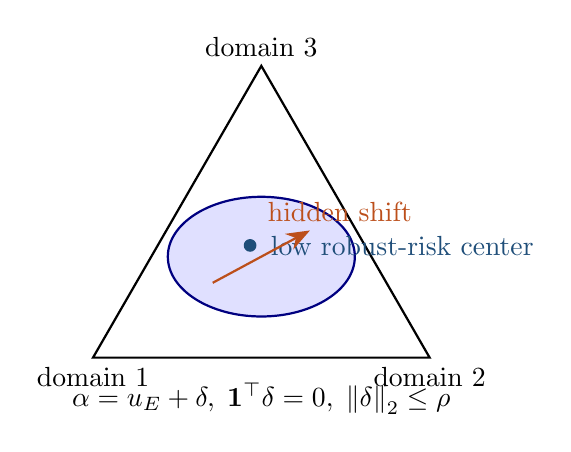
\begin{tikzpicture}[scale=0.95]
\draw[thick] (0,0) -- (4.5,0) -- (2.25,3.9) -- cycle;
\node[below] at (0,0) {domain 1};
\node[below] at (4.5,0) {domain 2};
\node[above] at (2.25,3.9) {domain 3};
\draw[fill=blue!12, draw=blue!50!black, thick] (2.25,1.35) ellipse (1.25 and 0.8);
\filldraw[accent] (2.1,1.5) circle (2.2pt) node[right=4pt] {low robust-risk center};
\draw[-{Stealth[length=3mm]}, thick, accent3] (1.6,1.0) -- (2.9,1.7);
\node[accent3] at (3.3,1.95) {hidden shift};
\node at (2.25,-0.55) {$\alpha = \ubar + \delta,\; \1^\top\delta=0,\; \norm{\delta}_2\le \rho$};
\end{tikzpicture}
\caption{Local source-mixture ambiguity around the nominal source mixture.}
\end{subfigure}
\hfill
\begin{subfigure}[t]{0.48\linewidth}
\centering
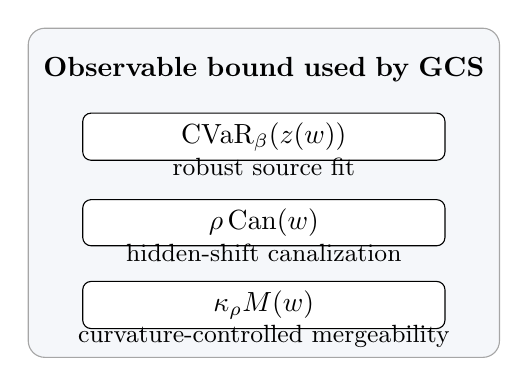
\begin{tikzpicture}[scale=0.95]
\draw[rounded corners=6pt, fill=softgray, draw=gray!70] (0,0) rectangle (6.3,4.4);
\node[align=center, text width=5.6cm] at (3.15,3.85) {\textbf{Observable bound used by GCS}};
\node[draw, rounded corners=3pt, fill=white, minimum width=4.6cm, minimum height=0.55cm] at (3.15,2.95) {$\cvar_{\beta}(z(w))$};
\node[font=\small] at (3.15,2.55) {robust source fit};
\node[draw, rounded corners=3pt, fill=white, minimum width=4.6cm, minimum height=0.55cm] at (3.15,1.8) {$\rho\operatorname{Can}(w)$};
\node[font=\small] at (3.15,1.4) {hidden-shift canalization};
\node[draw, rounded corners=3pt, fill=white, minimum width=4.6cm, minimum height=0.55cm] at (3.15,0.7) {$\kappa_{\rho}M(w)$};
\node[font=\small] at (3.15,0.28) {curvature-controlled mergeability};
\end{tikzpicture}
\caption{The practical objective is one convex optimization over the full bank.}
\end{subfigure}
\caption{Theory visualization. Left: the theorem-bearing hidden-shift ambiguity set. Right: the three-term GCS upper bound that becomes the method.}
\end{figure}

\begin{figure}[p]
\centering
\begin{subfigure}[t]{0.49\linewidth}
\centering
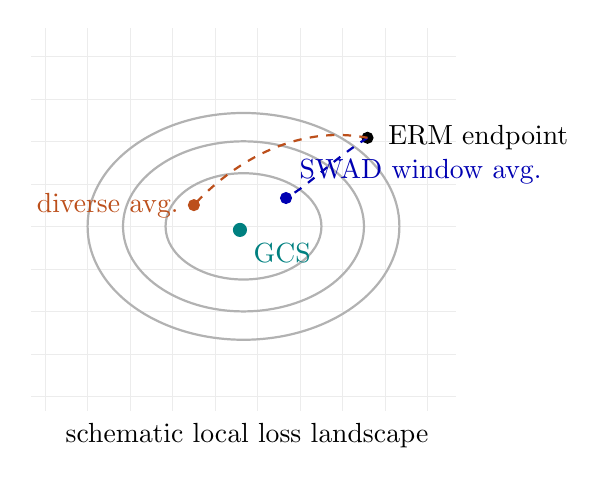
\begin{tikzpicture}[scale=0.9]
\draw[step=0.6, very thin, gray!15] (-0.2,-0.2) grid (5.8,5.2);
\draw[thick, gray!60] (2.8,2.4) ellipse (2.2 and 1.6);
\draw[thick, gray!60] (2.8,2.4) ellipse (1.7 and 1.2);
\draw[thick, gray!60] (2.8,2.4) ellipse (1.1 and 0.75);
\filldraw[black] (4.55,3.65) circle (2.2pt) node[right=4pt] {ERM endpoint};
\filldraw[blue!70!black] (3.4,2.8) circle (2.2pt) node[above right=2pt] {SWAD window avg.};
\filldraw[accent3] (2.1,2.7) circle (2.2pt) node[left=2pt] {diverse avg.};
\filldraw[accent2] (2.75,2.35) circle (2.6pt) node[below right=2pt] {GCS};
\draw[dashed, thick, blue!70!black] (4.55,3.65) .. controls (4.0,3.3) and (3.75,3.0) .. (3.4,2.8);
\draw[dashed, thick, accent3] (4.55,3.65) .. controls (3.5,3.85) and (2.6,3.25) .. (2.1,2.7);
\node at (2.85,-0.55) {schematic local loss landscape};
\end{tikzpicture}
\caption{Flatness and diversity become compatible when the final soup sits inside a low-curvature core.}
\end{subfigure}
\hfill
\begin{subfigure}[t]{0.49\linewidth}
\centering
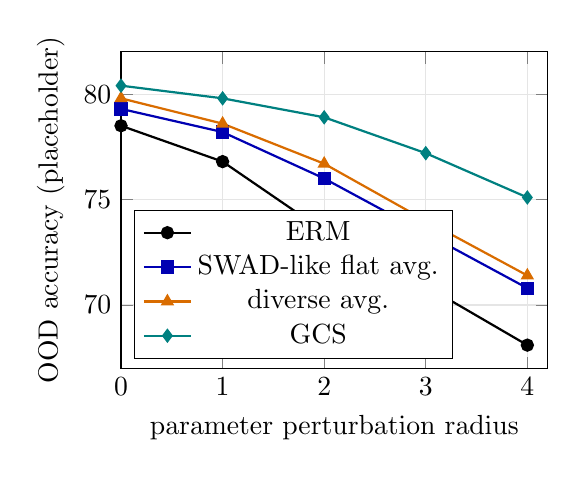
\begin{tikzpicture}
\begin{axis}[
    width=7cm, height=5.6cm,
    xmin=0,xmax=4.2,
    ymin=67,ymax=82,
    xlabel={parameter perturbation radius},
    ylabel={OOD accuracy (placeholder)},
    legend pos=south west,
    grid=major,
    grid style={gray!20},
]
\addplot[thick, black, mark=*] coordinates {(0,78.5) (1,76.8) (2,73.5) (3,70.9) (4,68.1)};
\addlegendentry{ERM}
\addplot[thick, blue!70!black, mark=square*] coordinates {(0,79.3) (1,78.2) (2,76.0) (3,73.4) (4,70.8)};
\addlegendentry{SWAD-like flat avg.}
\addplot[thick, orange!85!black, mark=triangle*] coordinates {(0,79.8) (1,78.6) (2,76.7) (3,74.0) (4,71.4)};
\addlegendentry{diverse avg.}
\addplot[thick, accent2, mark=diamond*] coordinates {(0,80.4) (1,79.8) (2,78.9) (3,77.2) (4,75.1)};
\addlegendentry{GCS}
\end{axis}
\end{tikzpicture}
\caption{Illustrative robustness curve: the target picture is that GCS stays stable as the perturbation radius grows.}
\end{subfigure}
\caption{Illustrative geometric and robustness explanations. These are not measured results.}
\end{figure}

\begin{figure}[p]
\centering
\begin{subfigure}[t]{0.48\linewidth}
\centering
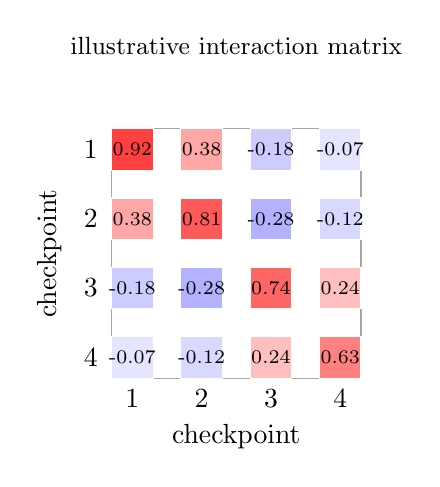
\begin{tikzpicture}[scale=0.88]
\node[font=\small] at (2.5,5.5) {illustrative interaction matrix};
\foreach \i/\lab in {1/1,2/2,3/3,4/4}{
  \node at (\i,0.4) {\lab};
  \node at (0.4,5-\i) {\lab};
}
\node at (2.5,-0.15) {checkpoint};
\node[rotate=90] at (-0.2,2.5) {checkpoint};
\draw[gray!70] (0.7,0.7) rectangle (4.3,4.3);
\def\cells{{1/4/red!75/0.92},{2/4/red!35/0.38},{3/4/blue!20/-0.18},{4/4/blue!10/-0.07},
{1/3/red!35/0.38},{2/3/red!65/0.81},{3/3/blue!30/-0.28},{4/3/blue!15/-0.12},
{1/2/blue!20/-0.18},{2/2/blue!30/-0.28},{3/2/red!60/0.74},{4/2/red!25/0.24},
{1/1/blue!10/-0.07},{2/1/blue!15/-0.12},{3/1/red!25/0.24},{4/1/red!50/0.63}}
\foreach \x/\y/\col/\val in \cells {
  \filldraw[fill=\col, draw=white] (\x-0.3,\y-0.3) rectangle (\x+0.3,\y+0.3);
  \node[font=\scriptsize] at (\x,\y) {\val};
}
\end{tikzpicture}
\caption{Negative off-diagonal entries represent complementary centered domain responses.}
\end{subfigure}
\hfill
\begin{subfigure}[t]{0.48\linewidth}
\centering
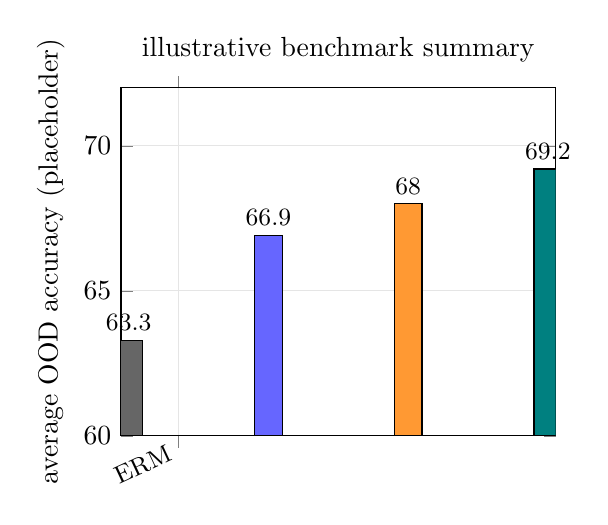
\begin{tikzpicture}
\begin{axis}[
    width=7.1cm, height=6cm,
    ybar, bar width=10pt,
    ymin=60, ymax=72,
    symbolic x coords={ERM,SWAD,DiWA,GCS},
    xtick=data,
    xticklabel style={rotate=25,anchor=east,font=\small},
    enlarge x limits=0.18,
    ylabel={average OOD accuracy (placeholder)},
    nodes near coords,
    every node near coord/.append style={font=\small},
    title={illustrative benchmark summary},
    grid=major, grid style={gray!20},
]
\addplot[fill=black!60] coordinates {(ERM,63.3)};
\addplot[fill=blue!60] coordinates {(SWAD,66.9)};
\addplot[fill=orange!80] coordinates {(DiWA,68.0)};
\addplot[fill=accent2] coordinates {(GCS,69.2)};
\end{axis}
\end{tikzpicture}
\caption{Placeholder benchmark panel. Real experiments would replace these numbers entirely.}
\end{subfigure}
\caption{Illustrative diversity and benchmark visuals.}
\end{figure}

\begin{table}[p]
\centering
\caption{Illustrative placeholder full-benchmark table. These values are fake and are included only to show expected paper layout.}
\vspace{0.4em}
\begin{tabular}{lcccccc}
\toprule
Method & PACS & VLCS & OfficeHome & TerraInc. & DomainNet & Avg. \\
\midrule
ERM & 85.5 & 77.5 & 66.5 & 46.1 & 40.9 & 63.3 \\
SWAD & 88.1 & 79.1 & 70.6 & 50.0 & 46.5 & 66.9 \\
DiWA & 89.0 & 78.6 & 72.8 & 51.9 & 47.7 & 68.0 \\
\textbf{GCS (placeholder)} & \textbf{89.7} & \textbf{79.9} & \textbf{73.6} & \textbf{52.8} & \textbf{50.0} & \textbf{69.2} \\
\bottomrule
\end{tabular}
\end{table}

\begin{table}[p]
\centering
\caption{Illustrative placeholder ablation table. Values are fake and only illustrate what the final empirical section could look like.}
\vspace{0.4em}
\begin{tabular}{lc}
\toprule
Variant & Avg. OOD accuracy (placeholder) \\
\midrule
GCS full & 69.2 \\
without canalization term & 68.2 \\
without curvature buffer & 67.7 \\
pooled mean instead of source-domain CVaR & 68.4 \\
uniform-on-support rather than optimized weights & 68.8 \\
\bottomrule
\end{tabular}
\end{table}

\section{Conclusion}
We presented a local, assumption-explicit theory from which major empirical intuitions about post-hoc DG emerge in a smooth regime. The theorem-bearing premise is that the deployable model should be robust to small signed tangent perturbations of source-mixture weights, and in sufficiently local feasible regimes to literal redistributions of source-support mass. This yields an exact hidden-shift support-function identity and a target-side held-out-loss upper bound in terms of mean source loss and source-mixture sensitivity under a fixed target-side envelope assumption. A principled strengthening of source fit is provided by source-domain CVaR. A practical deployable soup method follows by comparing the true soup to the observable checkpoint bank through local second-order geometry around a fixed prototype. The resulting GCS objective is one global convex optimization over the entire checkpoint bank, requiring no retained-family search, but its mergeability coefficient is theory-motivated rather than fully observable because it depends on local curvature constants. Diversity appears as negative centered interaction in the squared canalization law; flatness appears as a small curvature buffer. In this way, the theory provides a coherent local explanatory lens under which flat averaging methods and diversity-seeking methods can both succeed, without claiming an unconditional theorem of domain generalization.

\begin{thebibliography}{99}
\bibitem{gulrajani2021domainbed}
Ishaan Gulrajani and David Lopez-Paz.
\newblock In search of lost domain generalization.
\newblock In \emph{International Conference on Learning Representations}, 2021.

\bibitem{cha2021swad}
Junbum Cha, Sanghyuk Chun, Kyungjae Lee, Han-Cheol Cho, Seunghyun Park, Yunsung Lee, and Sungrae Park.
\newblock SWAD: Domain generalization by seeking flat minima.
\newblock In \emph{Advances in Neural Information Processing Systems}, 2021.

\bibitem{rame2022diwa}
Alexandre Ram\'e, Matthieu Kirchmeyer, Thibaud Rahier, Alain Rakotomamonjy, Patrick Gallinari, and Matthieu Cord.
\newblock Diverse weight averaging for out-of-distribution generalization.
\newblock In \emph{Advances in Neural Information Processing Systems}, 2022.

\bibitem{garipov2018connectivity}
Timur Garipov, Pavel Izmailov, Dmitrii Podoprikhin, Dmitry Vetrov, and Andrew Gordon Wilson.
\newblock Loss surfaces, mode connectivity, and fast ensembling of DNNs.
\newblock In \emph{Advances in Neural Information Processing Systems}, 2018.

\bibitem{frankle2020connectivity}
Jonathan Frankle, Gintare Karolina Dziugaite, Daniel Roy, and Michael Carbin.
\newblock Linear mode connectivity and the lottery ticket hypothesis.
\newblock In \emph{International Conference on Machine Learning}, 2020.

\bibitem{wortsman2022soups}
Mitchell Wortsman, Gabriel Ilharco, Samir Yitzhak Gadre, Rebecca Roelofs, Raphael Gontijo-Lopes, Ali Farhadi, Yair Carmon, Simon Kornblith, and Ludwig Schmidt.
\newblock Model soups: averaging weights of multiple fine-tuned models improves accuracy without increasing inference time.
\newblock In \emph{International Conference on Machine Learning}, 2022.
\end{thebibliography}

\end{document}
